\begin{figure}[htb!]
\begin{center}
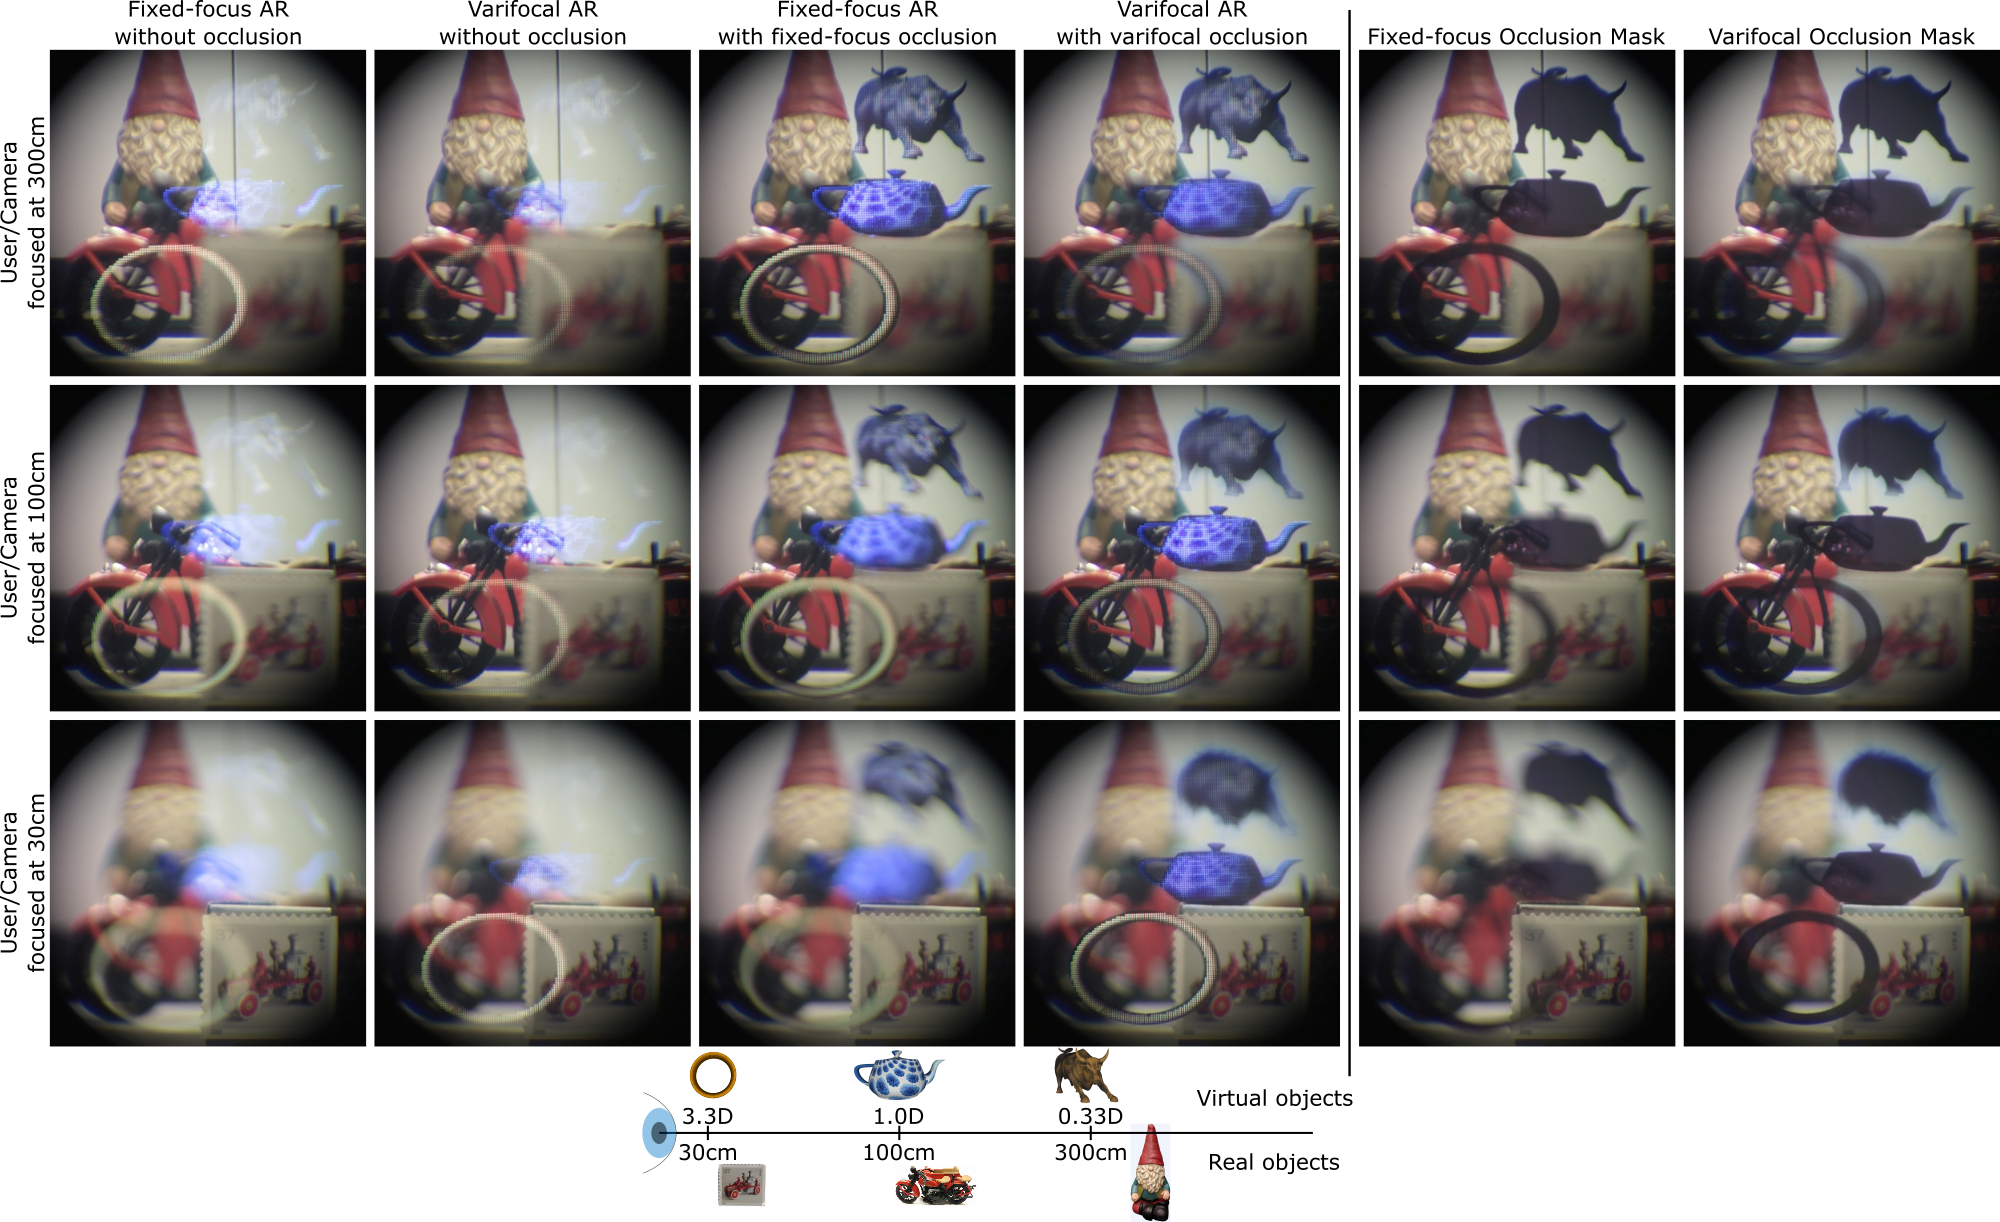
\includegraphics[width=0.9\textwidth]{images/volumetric/distortion_correction/results}
\end{center}
\caption[Volumetric NED: Results of optical calibration and distortion correction]{Demonstration of our calibration and distortion-correction approach. For these images, the display is displaying a volume across a large depth-range (15 cm to 400 cm). To ensure that all the images in this large depth-range are clearly visible, the aperture of the camera was set to the smallest setting. The chromatic artifacts seem to occur only for this narrow aperture setting.}
\label{fig:volumetric:distortion_correction:results} 
\end{figure} 
